% !TEX root = epifanov_solid_state_physics.tex
%!TEX TS-program = pdflatex
%!TEX encoding = UTF-8 Unicode


\chapter[Elements of Physical Statistics]{Elements of Physical Statistics}\label{chap:3}
% \chaptermark{Bonding. The Internal Structure of Solids}

Every solid is a system, or an ensemble, consisting of an enormous number of microscopic particles. Such systems obey specific \textit{statistical laws}, which are the subject of statistical physics, or physical statistics.

The present chapter deals briefly with the principal elements of physical statistics needed to describe the properties of solids.

\section{Methods used to describe the state of a macroscopic system}\label{sec:23}

There are two methods of describing the state of a system consisting of a great number of microscopic particles, the \textit{thermodynamic} and the \textit{statistical} method. Let us discuss them.

\textbf{Thermodynamic description of a system.} In the thermodynamic approach to the description of the state of a system consisting of an enormous number of particles the latter is regarded as a macroscopic system, it being of no interest of what type of particles it consists. Such a system is termed a \textit{thermodynamic system}.

A thermodynamic system may be either \textit{closed} or \textit{open}. A closed system does not interact in any way with the surroundings, and an open system can exchange heat and/or work with the surroundings.

The state of a system in which it can remain infinitely long is termed the \textit{equilibrium state}. It is uniquely determined by a set of independent physical parameters, the \textit{state parameters}. The principal state parameters are the \textit{volume} of the system $V$, the \textit{pressure} $p$, and the \textit{temperature} $T$. However, often those parameters are inadequate for a complete characteristic of the system. For a system made up of several substances one has also to know their concentrations; for a system in an electric or a magnetic field the intensities of these fields should be specified; etc.

Any change in a thermodynamic system involving the variation of at least one state parameter is termed a \textit{thermodynamic process}.

The sum of all types of energy of a closed system is termed the \textit{internal energy} ($E$) of the system. It is made up of the kinetic energy of the particles constituting the system, of the potential energy of the interaction between the particles, and of the internal energy of the particles themselves (which shall not be considered here since it is not subject to change in usual processes).

The internal energy is a \textit{function of state} of the system. This means that there is one and only one definite value of internal energy that corresponds to each state no matter how the system arrived at this
state.

Interacting with the surroundings a thermodynamic system may receive or reject some amounts $\Delta{Q}$ of heat, may perform work $\Delta{A}$ or have work performed on it. In all cases the variation in internal energy of the system, $\deriv{E}$, should be equal to the difference in the amount of heat received from outside, $\Delta{Q}$, and the work $\Delta{A}$ performed by the system against external forces:
\begin{equation}\label{eq:3_1}
    \deriv{E} = \Delta{Q} - \Delta{A}.
\end{equation}

\noindent
This is the first law of thermodynamics.

It should be pointed out that in contrast to the internal energy the work $\Delta{A}$ and the amount of heat $\Delta{Q}$ depend not only on the initial and the final states of the system but on the way the state is changed as well. Since
\begin{equation}\label{eq:3_2}
    \Delta{A} = p\, \deriv{V}
\end{equation}

\noindent
where $\deriv{V}$ is the variation of the volume of the system the pressure in which is $p$, we may write \eqref{eq:3_1} in the form
\begin{equation}\label{eq:3_3}
    \deriv{E} = \Delta{Q} - p\, \deriv{V}.
\end{equation}

The second law of thermodynamics maintains that the amount of heat $\Delta{Q}$ received by the system in a reversible process results in the increase of the entropy of the system by
\begin{equation}\label{eq:3_4}
    \deriv{S} = \frac{\Delta{Q}}{T}
\end{equation}

\noindent
where $T$ is the temperature at which the heat is received. Substituting $\Delta{Q}$ from \eqref{eq:3_4} into \eqref{eq:3_3}, we obtain
\begin{equation}\label{eq:3_5}
    \deriv{E} = T\, \deriv{S} - p\, \deriv{V}.
\end{equation}

\noindent
It follows from \eqref{eq:3_5} that the system's internal energy can be changed at the expense of work performed or heat exchanged.

However, the system's energy may also change with the change in the number of particles it contains, for every particle leaving the system takes away a definite amount of energy with it. Therefore, the general expression for the law of conservation of energy \eqref{eq:3_5} should
be written in the form
\begin{equation}\label{eq:3_6}
    \deriv{E} = T\, \deriv{S} - p\, \deriv{V} + \mu\, \deriv{N}
\end{equation}

\noindent
where $\deriv{N}$ is the variation of the number of particles in the system. Parameter $\mu$ is termed the \textit{chemical potential} of the system. Its physical meaning is as follows. For an isolated system of constant volume which neither receives nor gives away heat, $\deriv{S}=\Delta{Q}/T=0$ and $\deriv{V}=0$. For such a system
\begin{equation}\label{eq:3_7}
    \deriv{E} = \mu\, \deriv{N}.
\end{equation}

\noindent
Whence
\begin{equation}\label{eq:3_8}
    \mu = \diff{E}{N}.
\end{equation}

Hence, the chemical potential expresses the variation of the energy of an isolated system of a constant volume brought about by a unit variation in the number of particles it contains.

Let us consider the conditions of equilibrium of a system whose total number of particles remains constant but the particles can go over from one body belonging to the system to another. Two electron conductors, for instance, two metals, in contact with each other at a constant temperature may serve as an example of such a system. Denote the chemical potential of the electron gas in the first metal by $\mu_1$ and in the second by $\mu_2$. Suppose $\deriv{N}$ electrons flow from one metal to another. According to \eqref{eq:3_7} this will reduce the energy of the first metal by $\deriv{E}_1=\mu_1\,\deriv{N}$ and increase the energy of the second by $\deriv{E}_2=\mu_2\,\deriv{N}$. For the metals to be in a state of equilibrium the necessary condition is
\begin{equation*}
    \deriv{E}_1 = \deriv{E}_2,\quad \text{or}\quad \mu_1\,\deriv{N} = \mu_2\,\deriv{N}.
\end{equation*}

\noindent
Hence the condition of equilibrium is
\begin{equation}\label{eq:3_9}
    \mu_1 = \mu_2.
\end{equation}

\noindent
This condition is valid not only in the case of two electron conductors in contact with each other but for any phases in contact with each other: the solid and the liquid, the liquid and the gaseous, etc. \textit{In all cases the condition of equilibrium is the equality of the chemical potentials}.

\textbf{Statistical method of describing a system.} To describe the state of every particle one should specify its three coordinates and three components of the momentum. Apparently, if one was to write the equations of motions of the particles and solve them, he would be able to obtain complete information on the behaviour of the system and to predict its state at any moment of time. Such calculations, however, are not only extremely tedious but, in fact, useless. The complexity of the problem stems from the fact that to describe the behaviour of the gas molecules normally contained in \SI{1}{\metre\cubed} one would have to solve about \num{e26} interconnected equations of motion and also take into account the initial conditions, which is practically impossible. Should such calculations be carried out, they would be of no value since the properties of a system in the state of equilibrium not only are independent of the initial values of the coordinates and of the momentum components but generally remain constant in time, although the coordinates and the momenta of the particles do change. It follows from here that there is a qualitative distinction between the system and the individual particles and that the behaviour of the former is governed by laws different from those that govern the behaviour of individual particles. These laws are the statistical laws. The following examples are proof of their existence.

The velocity of an individual gas molecule is a random quantity, which is impossible to predict. Despite this fact, in a gas with a very large number of particles, on the average a distinct velocity distribution of its molecules may be observed. In other words, on the average a quite definite fraction of the molecules has a speed of, say, from \SIrange{100}{200}{\metre\per\second}, from \SIrange{400}{500}{\metre\per\second}, etc.

It is a matter of chance whether or not a given molecule shall enter a specified volume of the gas. Despite this fact there is a definite regularity in the distribution of the molecules over the volume: equal elements of volume contain, on the average, equal numbers of molecules.

The situation here is similar to that when a coin is tossed. The landing of the coin heads or tails up is a random event. Nevertheless, when the number of times the coin is tossed is very great, a quite definite regularity may be observed: on the average, the coin lands heads up half the number of times.

Such regularities are termed \textit{statistical}. The principal feature of statistical laws is that they deal with \textit{probabilities}. They enable predictions to be made only as to the probability of some event occurring or some result being realized. In the example with the coin the predicted probability of the coin landing one or the other side up is $1/2$. The results of individual tests may, and undoubtedly shall, deviate from those values the more the less the number of tests is. If we toss a coin five times, the head may fall out any number of times from $0$ to $5$. But the greater the number of tosses, that is, the more numerous the ensemble, the more accurate the statistical predictions are. Calculations show the relative deviation of an observed physical quantity (for instance, of the number of particles per unit volume) from the average value $\overline{M}$ in a system of $N$ noninteracting particles to be
\begin{equation*}
    \frac{\sqrt{\Delta{M}^2}}{\overline{M}} \propto \frac{1}{\sqrt{N}}
\end{equation*}

\noindent
or inversely proportional to $\sqrt{N}$.

As $N$ is increased, the ratio $\Delta{M}/\overline{M}\to 0$. For very great $N$ we have that $M/\overline{M}\approx 1$. Thus \SI{1}{\metre\cubed} of air normally contains on the average \num{2.7e25} molecules. The relative deviation from this number is on the average equal to
\begin{equation*}
    \frac{100\%}{\sqrt{N}} \approx \num{2e-11}\%.
\end{equation*}

\noindent
This deviation is so negligible that there are no instruments capable of detecting it. Therefore when dealing with large volumes it is always reasonable to assume that the distribution of molecules over the volume is uniform.

It should, however, be pointed out that deviations from the average values are not a possibility but a necessity. Such deviations are termed \textit{fluctuations}.

\section{Degenerate and nondegenerate ensembles}\label{sec:24}

\textbf{Microscopic particles and the ensemble.} All microscopic particles making up an ensemble may be subdivided into two classes according to their behaviour: fermions and bosons.

\textit{Fermions} include electrons, protons, neutrons and other particles with a half-odd integral values of spin: $\hslash/2, 3\hslash/2,\ldots$. Bosons include photons, phonons and other particles with integral values of spin: $0, \hslash, 2\hslash, \ldots$.

The fermions in an ensemble exhibit marked ``individualistic'' tendencies. If some quantum state is already occupied by a fermion, no other fermion shall settle in it. This is the essence of the well-known \textit{Pauli exclusion principle}, which governs the behaviour of fermions. Bosons, on the other hand, strive for ``unification''. They can settle in the same state in any numbers and do it the more readily the more populated the state already is.

\textit{Degenerate and nondegenerate ensembles.} Let us discuss the possible effects of the nature of the particles (their fermionic or bosonic character) on the properties of the ensemble as a whole.

For the nature to be felt the particles must ``meet'' often enough. This means that they must occupy the same state or at least sufficiently closely-spaced states.

Suppose that there are $G$ different states which any one of $N$ similar particles can occupy. The ratio $N/G$ may serve as a measure of the ``meeting'' frequency. The meetings will be rare if
\begin{equation}\label{eq:3_10}
    \frac{N}{G}\gg 1.
\end{equation}

\noindent
In this case the number of different vacant states is much larger than the number of particles: $G\gg N$. Evidently, in such circumstances the specific nature of fermions and bosons shall not be felt, since every particle has at its disposal a large number of different free states and the problem of several particles occupying the same state actually does not arise. Therefore, the properties of the ensemble as a whole shall not depend on the nature of the particles that make it up. Such ensembles are termed \textit{nondegenerate}, and condition \eqref{eq:3_10} is the \textit{condition of nondegeneracy}.

If, however, the number of states $G$ is of the same order of magnitude as the number of particles $N$, that is if
\begin{equation}\label{eq:3_11}
    \frac{N}{G}\approx 1
\end{equation}

\noindent
then the problem of how the states should be occupied, whether individually or collectively, indeed assumes much importance. In this case the nature of the microscopic particle is fully revealed in its effect on the properties of the ensemble as a whole. Such ensembles
are termed \textit{degenerate}.

Degenerate ensembles are a unique property of quantum objects, since the parameters of state of such objects only change discretely with the result that the number of possible states $G$ can be finite. The number of states for classical objects whose parameters change continuously is always infinite and they can form only nondegenerate ensembles.

It should be pointed out that quantum mechanical objects too may form nondegenerate ensembles provided condition \eqref{eq:3_10} is fulfilled (see \tab{3_1}).

\begin{table}[!b]
	\renewcommand{\arraystretch}{1.2}
	\caption{}
	\vspace{-0.6cm}
	\label{table:3_1}
	\begin{center}\resizebox{0.6\linewidth}{!}{
			\begin{tabular}{lll}
				\toprule[1pt]
				\multirow{2}{*}{\textbf{Object}} & \multicolumn{2}{c}{\textbf{Ensembles}} \\
                \cline{2-3}
                & \textbf{Degenerate} & \textbf{Nondegenerate}\\
				\midrule[0.5pt]\midrule[0.5pt]
				Classical & No & Yes\\
                Quantum & Yes & Yes\\
				\bottomrule[1pt]
			\end{tabular}
	}\end{center}
\end{table}

\textbf{Classical and quantum statistics.} Physical statistics that studies nondegenerate ensembles is termed \textit{classical statistics}. It owes much to J. C. Maxwell and L. E. Boltzmann (the \textit{Maxwell-Boltzmann statistics}).

Physical statistics that studies degenerate ensembles is termed \textit{quantum statistics}. Owing to the effect of the particles' nature on the properties of a degenerate ensemble, degenerate ensembles of fermions and bosons behave in essentially different ways. On this ground a distinction is made between two quantum statistics.

Quantum statistics of fermions owes much to E. Fermi and P. A. M. Dirac (this, by the way, explains the origin of the term ``fermion''). It is termed the \textit{Fermi-Dirac statistics}.

Quantum statistics of bosons owes much to S. N. Bose and A. Einstein (hence the term ``boson''). It is termed the \textit{Bose-Einstein statistics}.

It follows then that quantum statistics deals only with quantum objects while classical statistics may deal both with the classical and the quantum objects. If we reduce the number of particles in an ensemble or increase the number of states, we shall eventually turn a degenerate ensemble into a nondegenerate one. In that case the ensemble shall be described by the Maxwell-Boltzmann statistics no matter whether it contains fermions or bosons.

\textbf{Distribution function.} What is the connection between the distribution of the particles over particular states and the state of the ensemble as a whole? To specify the state of an ensemble, for instance, of a gas of particles, one should specify its state parameters. To specify the state of each particle one should specify its coordinates and momentum components or its energy, which is a function of coordinates and momentum.

The two types of quantities are connected by the \textit{statistical distribution function}
\vspace{-12pt}
\begin{equation}\label{eq:3_12}
    N_{\mu,T}(E)\,\deriv{E}
\end{equation}

\noindent
which specifies the number of particles having an energy from $E$ to
$E+\deriv{E}$ in the system described by the state parameters $\mu$ and $T$.

This function is termed \textit{complete statistical distribution function}. To simplify notation the indices denoting the state parameters are usually omitted.

The complete distribution function may be represented by the product of the number of states $g(E)\,\deriv{E}$ per energy interval $\deriv{E}$ and the probability of occupation of those states by the particles. Let us denote the latter by $f(E)$. Then
\begin{equation}\label{eq:3_13}
    N(E)\,\deriv{E} = f(E) g(E)\, \deriv{E}.
\end{equation}

The function $f(E)$ is termed simply the \textit{distribution function}. As was stated before it signifies the probability of the occupation of the respective states by the particles. If, for instance, $10$ of $100$ closely spaced states are occupied by particles (the total number of particles in the system being much greater than $100$), the probability of occupation of such states will be equal to $0.1$. Since on the average there is $0.1$ of a particle per each state, we may take $f(E)$ to be the average number of particles in a given state.

Hence, the problem of finding the complete distribution function of particles over the states is reduced to that of finding the function $g(E)\,\deriv{E}$, which describes the energy distribution of the states, and the function $f(E)$ which determines the probability of their occupation.

We start by determining the function $g(E)\,\deriv{E}$.

\section{The number of states for microscopic particles}\label{sec:25}

\textbf{Concept of phase space of a microscopic particle and quantization.} In classical mechanics the state of a particle is determined if its three coordinates ($x, y, z$) and three components of its momentum ($p_x, p_y, p_z$) are specified. Let us imagine a six-dimensional space with the coordinate axes $x, y, z, p_x, p_y, p_z$. The state of the particle at every moment of time will be described by a point ($x, y, z, p_x, p_y, p_z$). Such space is termed \textit{phase space} and the points ($x, y, z, p_x, p_y, p_z$) are termed \textit{phase points}. The quantity
\begin{equation}\label{eq:3_14}
    \Delta{\Gamma} = \Delta{\Gamma}_V \Delta{\Gamma}_p = \deriv{x}\,\deriv{y}\,\deriv{z}\, \deriv{p_x}\,\deriv{p_y}\,\deriv{p_z}
\end{equation}

\noindent
is termed an element of the phase space. Here, $\Delta{\Gamma}_V=\deriv{x}\,\deriv{y}\,\deriv{z}$ is an element of volume in coordinate space and $\Delta{\Gamma}_p=\deriv{p_x}\,\deriv{p_y}\,\deriv{p_z}$ an element of volume in momentum space.

Since the coordinates and the momentum components of a classical particle may change continuously, the elements $\Delta{\Gamma}_V, \Delta{\Gamma}_p$ and with them the element $\Delta{\Gamma}$ as well can be chosen as small as desired.

The potential energy of a system of noninteracting particles not acted upon by an external field is zero. Such particles are termed \textit{free}. For such particles it is convenient to use a three-dimensional momentum space instead of the six-dimensional phase space. In this case, the element $\Delta{\Gamma}_V$ is simply equal to the volume $V$ in which the particles move, because no additional restrictions are placed on them.

The division of the phase space into elements of volume is not quite so simple if the particle in question is an electron or some other microscopic object possessing wave properties. The wave properties of such particles make it impossible, in accordance with the uncertainty principle, to distinguish between two states, ($x, y, z, p_x, p_y, p_z$) and ($x+\deriv{x}, y+\deriv{y}, z+\deriv{z}, p_x+\deriv{p_x}, p_y+\deriv{p_y}, p_z+\deriv{z}$), if the product $\deriv{x}\,\deriv{y}\,\deriv{z}\, \deriv{p_x}\,\deriv{p_y}\,\deriv{p_z}$ is less than $h^3$. Since this product represents an element of volume in six-dimensional phase space, it follows from the above that different quantum states shall correspond to different elements of volume in this space only if the size of those elements is no less than $h^3$. Therefore quantum statistics makes use of an elementary cell in the six-dimensional space with the volume
\begin{equation}\label{eq:3_15}
    \Delta{\Gamma} = \Delta{\Gamma}_V \Delta{\Gamma}_p = h^3.
\end{equation}

\noindent
The element of the three-dimensional momentum space for free particles for which $\Delta{\Gamma}_V=V$ is
\begin{equation}\label{eq:3_16}
    \Delta{\Gamma}_p = \frac{h^3}{V}.
\end{equation}

\noindent
Each element of this kind has corresponding to it a definite quantum state.

The process of dividing the phase space into cells of finite size ($h^3$ or $h^3/V$) is termed \textit{quantization of phase space}.

\textbf{Density of states.} We wish to calculate the number of states of a free particle in the energy interval from $E$ to $E+\deriv{E}$. To this end draw two spheres of the radii $p$ and $p\deriv{p}$ in the momentum space (\fig{3_1}). There is a spherical layer with the volume of $4\pi p^2\,\deriv{p}$ contained between the spheres. The number of phase cells contained in this layer is
\begin{equation}\label{eq:3_17}
    \frac{4\pi p^2\, \deriv{p}}{\Delta{\Gamma}_p} = \frac{4\pi V}{h^3}p^2\, \deriv{p}.
\end{equation}

\begin{figure}[t]
	\begin{center}
		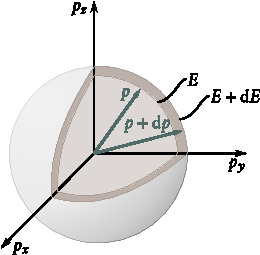
\includegraphics[scale=1]{figures/ch_03/fig_3_1.pdf}
		\caption[]{Calculating the number of states of a microscopic particle.}
		\label{fig:3_1}
	\end{center}
	\vspace{-0.7cm}
\end{figure}

Since there is one particle state to correspond to every cell the number of states in the interval $\deriv{p}$ between $p$ and $p+\deriv{p}$ is
\begin{equation}\label{eq:3_18}
    g(p)\,\deriv{p} = \frac{4\pi V}{h^3}p^2\, \deriv{p}.
\end{equation}

For free (noninteracting) particles
\begin{equation*}
    E = \frac{p^2}{2m},\quad \deriv{E} = \frac{p}{m}\,\deriv{p}.
\end{equation*}

\noindent
Using these relations to express $p$ and $\deriv{p}$ and substituting the results into \eqref{eq:3_18}, we obtain
\begin{equation}\label{eq:3_19}
    g(E)\,\deriv{E} = \frac{2\pi V}{h^3}(2m)^{3/2} E^{1/2}\, \deriv{E}.
\end{equation}

\noindent
This is the number of states of a free particle in the energy interval ($E, E+\deriv{E}$). Dividing the right- and the left-hand sides of \eqref{eq:3_19} by $\deriv{E}$, we obtain the density of states, $g(E)$, which specifies the number of states of a microscopic particle per unit energy interval:
\begin{equation}\label{eq:3_20}
    g(E) = \frac{2\pi V}{h^3}(2m)^{3/2} E^{1/2}.
\end{equation}

It follows from \eqref{eq:3_20} that as $E$ increases the density of states rises in proportion to $E^{1/2}$ (\fig{3_2}). The density of states depends, besides, on the particle's mass and increases with $m$.

\begin{figure}[t]
	\begin{center}
		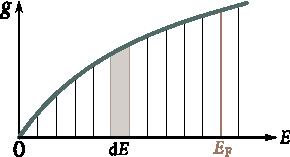
\includegraphics[scale=1]{figures/ch_03/fig_3_2.pdf}
		\caption[]{Energy dependence of density of states.}
		\label{fig:3_2}
	\end{center}
	\vspace{-0.7cm}
\end{figure}

In case of the electrons each phase cell corresponds, to be exact, not to one but to two states, each distinguished by its spin. They are termed \textit{spin states}. Therefore, in case of the electrons the number of states \eqref{eq:3_18} and \eqref{eq:3_19} and the density \eqref{eq:3_20} should be doubled:
\begin{align}
    g(p)\, \deriv{p} &= \frac{8\pi V}{h^3} p^2\,\deriv{p},\label{eq:3_21}\\
    g(E)\, \deriv{E} &= \frac{4\pi V}{h^3} (2m)^{3/2} E^{1/2}\,\deriv{E},\label{eq:3_22}\\
    g(E) &= \frac{4\pi V}{h^3} (2m)^{3/2} E^{1/2}.\label{eq:3_23}
\end{align}

\textbf{Condition of nondegeneracy for an ideal gas.} Integrating \eqref{eq:3_20} with respect to energy from $0$ to $E$, we obtain the number of particle states contained within the energy interval ($0, E$):
\begin{equation*}
    G = \frac{2\pi V}{h^3} (2m)^{3/2} \frac{2}{3} E^{3/2}.
\end{equation*}

\noindent
Setting $E=3\ab{k}{B}T/2$, we obtain
\begin{equation*}
    G \approx V \parenthesis{\frac{2\pi m \ab{k}{B} T}{h^2}}^{3/2}.
\end{equation*}

\noindent
Substituting this expression into \eqref{eq:3_10}, we obtain the condition for nondegeneracy:
\vspace{-12pt}
\begin{equation}\label{eq:3_24}
    n \parenthesis{\frac{h^2}{2\pi m \ab{k}{B} T}}^{3/2} \ll 1
\end{equation}

where $n=N/V$ is the number of particles per unit volume.

Consider some molecular gas, for instance, nitrogen in normal conditions. For it $n\approx\SI{e26}{\per\metre\cubed}$, $m=\SI{4.5e-26}{\kilo\gram}$, and $\ab{k}{B}T=\SI{4e-21}{\joule}$. Substituting the figures into the left-hand side of \eqref{eq:3_24}, we obtain $nh^3(2\pi m\ab{k}{B}T)^{-3/2}\approx\num{e-6}$, which is much less than unity. Accordingly, the molecular gases are normally nondegenerate and must be described with the aid of the Maxwell-Boltzmann classical statistics.

Consider now the electron gas in metals. For it we have that $n\approx\SI{5e24}{\per\metre\cubed}$ and $m=\SI{9e-31}{\kilo\gram}$. For such values of $n$ and $m$ the electron gas turns out to be nondegenerate only at temperatures above \SI{105}{\kelvin}; the left-hand side of \eqref{eq:3_24} for such temperatures diminishes to less than unity (at $T=\SI{105}{\kelvin}$ it is approximately $0.5$). Therefore, in practice the electron gas in metals is always degenerate and on account of this should be described with the aid of the Fermi-Dirac statistics.

It follows from \eqref{eq:3_24} that a nondegenerate state of a gas can be realized not only by raising its temperature but by reducing its concentration $n$ as well. For $n\approx\SI{e22}{\per\metre\cubed}$ the left-hand side of \eqref{eq:3_24} for electrons at normal temperatures is approximately \num{e-3} and the electron gas becomes nondegenerate. Such (and smaller) concentrations of the electron gas are found in some semiconductors. In such semiconductors termed \textit{nondegenerate}, the electron gas is nondegenerate and is described by the classical Maxwell-Boltzmann statistics.

Let us try now to find the distribution function $f(E)$. The form of this function depends in the first instance on whether the gas is degenerate or nondegenerate. In the case of a degenerate gas the important point is whether the gas consists of fermions or bosons.

Let us start with a nondegenerate gas whose distribution function $f(E)$ is independent of the particles' nature.

\section{Distribution function for a nondegenerate gas}\label{sec:26}

Appendix \ref{sec:A_I} contains an elementary derivation of the distribution function for a nondegenerate gas. It is of the following form:
\begin{equation}\label{eq:3_25}
    f(E) = e^{(\mu - E) / \ab{k}{B} T}
\end{equation}

\noindent
where $\ab{k}{B}$ is Boltzmann's constant, and $\mu$ the chemical potential. Calculations give the following expression for $\mu$ of a nondegenerate gas:
\begin{equation}\label{eq:3_26}
    \mu = \ab{k}{B} T \ln\bracket{\frac{N}{V} \parenthesis{\frac{h^2}{2\pi m \ab{k}{B} T}}^{3/2}}.
\end{equation}

Substituting it into \eqref{eq:3_25} we obtain:
\begin{equation}\label{eq:3_27}
    \ab{f}{M}(E) = \frac{N}{V} \parenthesis{\frac{h^2}{2\pi m \ab{k}{B} T}}^{3/2} e^{-E/(\ab{k}{B} T)}.
\end{equation}

\noindent
We would like to remind again that $\ab{f}{M}(E)\,\deriv{E}$ expresses the probability of occupation of the states in the energy interval ($E, E+\deriv{E}$); the term for it is the \textit{Maxwell-Boltzmann distribution function}.

Figure \fig{3_3}(a) shows a graph of the function $\ab{f}{M}(E)$. It has a maximum at $E=0$ and asymptotically approaches zero as $E\to\infty$. This means that the lower energy states have the greatest probability of occupation. As the energy of a state increases its probability of occupation diminishes steadily.

\begin{figure}[t]
	\begin{center}
		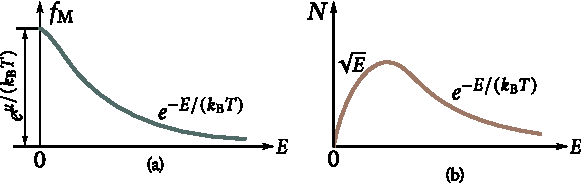
\includegraphics[scale=0.95]{figures/ch_03/fig_3_3.pdf}
		\caption[]{Distribution functions for nondegenerate gas: (a) ---the Maxwell-Boltzmann distribution function expressing the average density of state occupation by particles; (b) --- the complete Maxwell-Boltzmann distribution function.}
		\label{fig:3_3}
	\end{center}
	\vspace{-0.7cm}
\end{figure}

Multiplying $\ab{f}{M}(E)$ by the number of states $g(E)\,\deriv{E}$ [see \eqn{3_22}], we obtain the complete distribution function of particles over the energy
\begin{equation}\label{eq:3_28}
    \begin{split}
    N(E)\, \deriv{E} &= \frac{4\pi V}{h^3} (2m)^{3/2} e^{\mu/(\ab{k}{B} T)} e^{-E/(\ab{k}{B} T)} E^{1/2}\, \deriv{E},\quad \text{or}\\
    N(E)\, \deriv{E} &= \frac{2N}{\sqrt{\pi(\ab{k}{B} T)^3}} e^{-E/(\ab{k}{B} T)} E^{1/2}\, \deriv{E}.
    \end{split}
\end{equation}

\noindent
It is termed the \textit{complete Maxwell-Boltzmann distribution function}. Figure \ref{fig:3_3}(b) shows the graph of this function. Because of the factor $E^{1/2}$ its maximum is displaced to the right of the origin.

Knowing the distribution function $\ab{f}{M}(E)$ we may easily find the laws of distribution of the particles over the momentum, $N(p)\,\deriv{p}$, and over its components, $N(p_x,p_y,p_z)\,\deriv{p_x}\,\deriv{p_y}\,\deriv{p_z}$. We may also find them over the velocity, $N(v)\,\deriv{v}$, and over its components $N(v_x,v_y,v_z)\,\deriv{v_x}\,\deriv{v_y}\,\deriv{v_z}$ over one of the components of velocity, say $N(v_x)\,\deriv{v_x}$, etc. Those distributions are shown below
\begin{align}
    N(p) &= \frac{4\pi N}{(2\pi m \ab{k}{B} T)^{3/2}} e^{-p^2/(2m\ab{k}{B}T)} p^2, \label{eq:3_29}\\
    N(v) &= 4\pi N \parenthesis{\frac{m}{2\pi\ab{k}{B} T}}^{3/2} e^{mv^2/(\ab{k}{B} T)} v^2, \label{eq:3_30}\\
    N(p_x,p_y,p_z) &= N \parenthesis{\frac{N}{2\pi m\ab{k}{B} T}}^{3/2} e^{-\parenthesis{p_x^2+p_y^2+p_z^2}/(2m\ab{k}{B} T)}, \label{eq:3_31}\\
    N(v_x,v_y,v_z) &= N \parenthesis{\frac{m}{2\pi\ab{k}{B} T}}^{3/2} e^{-m\parenthesis{v_x^2+v_y^2+v_z^2}/(2\ab{k}{B} T)}, \label{eq:3_32}\\
    N(v_x) &= N \parenthesis{\frac{m}{2\pi\ab{k}{B} T}}^{1/2} e^{-mv_x^2/(2\ab{k}{B} T)}. \label{eq:3_33}
\end{align}

\noindent
The reader is requested to obtain those results himself.

\section{Distribution function for a degenerate fermion gas}\label{sec:27}

The distribution function for a degenerate fermion gas was first obtained by Fermi and Dirac. It is of the following form:
\begin{equation}\label{eq:3_34}
    \ab{f}{F}(E) = \frac{1}{e^{(E - \mu)/(\ab{k}{B} T)} + 1}.
\end{equation}

An elementary derivation of this expression is presented in Appendix \ref{sec:A_II}. Here, as before, $\mu$, denotes the chemical potential, which in the case of a degenerate fermion gas is termed the \textit{Fermi level}.

Equation \eqref{eq:3_34} shows that for $E=\mu$, the distribution function $f(E)=1/2$ at any temperature $T\neq 0$. Therefore, from the statistical point of view the Fermi level is a state whose probability of
occupation is $1/2$.

The function \eqref{eq:3_34} is termed the \textit{Fermi-Dirac function}. To obtain a clear picture of the nature of this function one should consider the degenerate electron gas in metals at absolute zero.

\begin{figure}[t]
	\begin{center}
		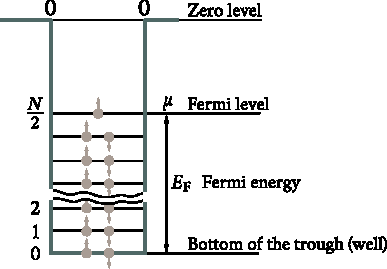
\includegraphics[scale=1]{figures/ch_03/fig_3_4.pdf}
		\caption[]{Schematic representation of a metal as a potential well for free electrons.}
		\label{fig:3_4}
	\end{center}
	\vspace{-0.7cm}
\end{figure}

\textbf{Electron distribution in a metal at absolute zero. Fermi energy.} The metal is a sort of a potential well (trough) for free electrons. To leave it the electron should have work performed on it against the forces retaining it in the metal. Figure \ref{fig:3_4} shows the diagram of such a potential well. The horizontal lines denote energy levels which the electrons may occupy. In compliance with the Pauli exclusion principle there may be two electrons with opposite spins on each such level. For an electron gas of $N$ electrons the last occupied level will be the $N/2$ level. This level is termed the \textit{Fermi level} for a degenerate electron gas. It corresponds to the maximum kinetic energy $\ab{E}{F}$ an electron in a metal may possess at absolute zero. This energy is termed the \textit{Fermi energy}.

Thus, at absolute zero all states with the energy $E<\ab{E}{F}$ are occupied by electrons and all states with the energy $E>\ab{E}{F}$ are free. In other words, the probability of occupation of a state with the energy $E<\ab{E}{F}$ at $T=\SI{0}{\kelvin}$ is unity and the probability of occupation of a state with the energy $E>\ab{E}{F}$ is zero:
\begin{equation}\label{eq:3_35}
    \ab{f}{F}(E) = \begin{cases}
    1,\quad \text{for}\quad E<\ab{E}{F},\\
    0,\quad \text{for}\quad E>\ab{E}{F}.
    \end{cases}
\end{equation}

To obtain this result from \eqref{eq:3_34} one should assume that at $T=\SI{0}{\kelvin}$ the chemical potential of the electron gas measured from the bottom of the potential well is equal to the Fermi energy $\ab{E}{F}$:
\begin{equation}\label{eq:3_36}
    \mu = \ab{E}{F}.
\end{equation}

\noindent
Indeed, setting in \eqref{eq:3_34} $\mu = \ab{E}{F}$ we obtain
\begin{equation}\label{eq:3_37}
    \ab{f}{F}(E) = \frac{1}{e^{(E - \ab{E}{F})/(\ab{k}{B} T)} + 1}.
\end{equation}

\noindent
If $E<\ab{E}{F}$, then $e^{(E - \ab{E}{F})/(\ab{k}{B} T)}\to 0$ at $T=\SI{0}{\kelvin}$ and $\ab{f}{F}=1$; if $E>\ab{E}{F}$, then $e^{(E - \ab{E}{F})/(\ab{k}{B} T)}\to\infty$ at $T=\SI{0}{\kelvin}$ and $\ab{f}{F}=0$.

Figure \ref{fig:3_5}(a) shows the graph of the Fermi-Dirac distribution function at absolute zero. It has the shape of a step terminating at $E=\ab{E}{F}$.

\begin{figure}[t]
	\begin{center}
		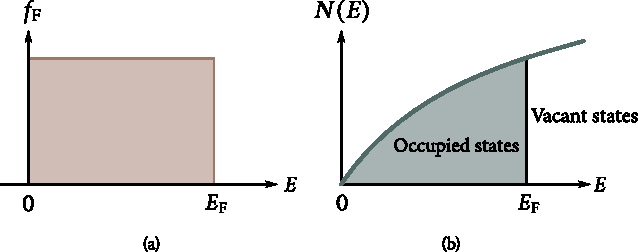
\includegraphics[scale=1]{figures/ch_03/fig_3_5.pdf}
		\caption[]{The distribution function for degenerate fermion gas: (a) --- the Fermi-Dirac distribution function for $T=\SI{0}{\kelvin}$; (b) --- the complete Fermi-Dirac distribution function for $T=\SI{0}{\kelvin}$.}
		\label{fig:3_5}
	\end{center}
	\vspace{-0.7cm}
\end{figure}

Multiplying \eqref{eq:3_35} by the number of states $g(E)\,\deriv{E}$ [see \eqn{3_22}], we obtain the \textit{complete Fermi-Dirac distribution function at absolute zero}:
\begin{equation}\label{eq:3_38}
    N(E)\, \deriv{E} = \frac{4\pi V}{h^3} (2m)^{3/2} E^{1/2}\, \deriv{E}
\end{equation}

\noindent
because $\ab{f}{F}=1$ in the energy interval ($0, \ab{E}{F}$). The graph of the function is presented in \fig{3_5}(b), where the area of the occupied states is shaded.

Integrating expression \eqref{eq:3_38} from $0$ to $\ab{E}{F}$, we obtain
\begin{equation*}
    N = \frac{8\pi V}{3h^3} \ab{E}{F}^{3/2} (2m)^{3/2}
\end{equation*}

\noindent
whence the Fermi energy may be easily obtained
\begin{equation}\label{eq:3_39}
    \ab{E}{F} = \frac{h^2}{2m} \parenthesis{\frac{3n}{8\pi}}^{2/3}
\end{equation}

\noindent
where $n=N/V$ is the concentration of electron gas in the metal.

Knowing the energy distribution function of the electrons, we may easily calculate the average energy of the electrons at absolute zero, $\overline{E}_0$:
\begin{equation}\label{eq:3_40}
    \overline{E}_0 = \frac{3}{5}\ab{E}{F} = \frac{3h^2}{10m} \parenthesis{\frac{3n}{8\pi}}^{2/3}.
\end{equation}

\noindent
Lastly, knowing $\ab{E}{F}$ and $\overline{E}_0$, we can calculate the maximum velocity $\ab{v}{F}$ and the effective velocity $\ab{v}{eff}$ (corresponding to average energy) of free electrons in a metal at absolute zero:
\begin{equation}\label{eq:3_41}
    \ab{v}{F} = \parenthesis{\frac{2\ab{E}{F}}{m}}^{1/2},\quad \ab{v}{F} = \parenthesis{\frac{2\overline{E}_0}{m}}^{1/2}.
\end{equation}

Table \ref{table:3_2} shows the Fermi energy $\ab{E}{F}$, the average energy $\overline{E}_0$, the maximum and effective velocities of free electrons at absolute zero for some metals. The last column contains the Fermi temperature determined from the relation
\begin{equation}\label{eq:3_42}
    \ab{T}{F} = \frac{\ab{E}{F}}{\ab{k}{B}}.
\end{equation}

\noindent
This is the temperature at which a molecule in a normal nondegenerate gas would have the energy of thermal motion $3\ab{k}{B}T/2$ equal to the Fermi energy $\ab{E}{F}$ multiplied by $3/2$.

\begin{table}[!b]
	\renewcommand{\arraystretch}{1.2}
	\caption{}
	\vspace{-0.6cm}
	\label{table:3_2}
	\begin{center}\resizebox{0.95\linewidth}{!}{
			\begin{tabular}{lccccc}
				\toprule[1pt]
				\textbf{Metal} & $\ab{E}{F}$ (\si{\electronvolt}) & $\overline{E}_0$ (\si{\electronvolt}) & $\ab{v}{F}\, \parenthesis{\SI{e6}{\metre\per\second}}$ & $\ab{v}{eff}\, \parenthesis{\SI{e6}{\metre\per\second}}$ & $\ab{T}{F}\, \parenthesis{\SI{e4}{\kelvin}}$\\
				\midrule[0.5pt]\midrule[0.5pt]
                Copper & $7.10$ & $4.30$ & $1.60$ & $1.25$ & $8.20$\\
                Lithium & $4.72$ & $2.80$ & $1.30$ & $1.00$ & $5.50$\\
                Silver & $5.50$ & $3.30$ & $1.40$ & $1.10$ & $6.40$\\
                Sodium & $3.12$ & $1.90$ & $1.10$ & $0.85$ & $3.70$\\
				\bottomrule[1pt]
			\end{tabular}
	}\end{center}
\end{table}

It may be seen from \tab{3_2} that Fermi temperatures are so high that no metal can exist in a condensed state.

It should be stressed that, although the Fermi energy represents the kinetic energy of translational motion of free electrons, it is not the energy of their thermal motion. Its nature is purely quantum mechanical and is due to the fact that electrons are fermions satisfying the Pauli exclusion principle.

\textbf{Temperature dependence of the Fermi-Dirac distribution.} When the temperature is raised, the electrons become thermally excited and go over to higher energy levels. This causes a change in their distribution over the states. However, in the range of temperatures in which the energy of their thermal motion, $\ab{k}{B}T$, remains much less than $\ab{E}{F}$ only the electrons in a narrow band about approximately $\ab{k}{B}T$ wide adjoining the Fermi level may be thermally excited [\fig{3_6}(a); the excited states are shaded]. The electrons of the lower levels remain practically unaffected because the energy of thermal excitation $\ab{k}{B}T$ is not enough to excite them (to transfer them to
levels above the Fermi level).

\begin{figure}[t]
	\begin{center}
		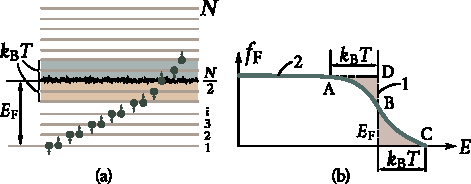
\includegraphics[scale=1.1]{figures/ch_03/fig_3_6.pdf}
		\caption[]{Temperature dependence of the Fermi-Dirac distribution function: (a) --- thermal excitation of electrons; (b) --- the Fermi-Dirac distribution function for $T>\SI{0}{\kelvin}$.}
		\label{fig:3_6}
	\end{center}
	\vspace{-0.7cm}
\end{figure}

As a result of thermal excitation some of the electrons with an energy less than $\ab{E}{F}$ are transferred to the levels with energies greater than $\ab{E}{F}$ and a new distribution of electrons over the states is established. Figure \ref{fig:3_6}(b) shows the curves of the electron distribution over the states for $T=\SI{0}{\kelvin}$ (curve $1$) and for $T>\SI{0}{\kelvin}$ (curve $2$). It can be seen that the rise in temperature causes the original distribution to smear to a depth of $\ab{k}{B}T$ with a ``tail'' BC appearing to the right of $\ab{E}{F}$. The higher the temperature the greater the change in the distribution function. The tail BC itself is described by the Maxwellian distribution function.

The shaded areas in \fig{3_6}(b) are proportional to the number of electrons transferred from the states with $E<\ab{E}{F}$ (the area ADB) to the states with $E>\ab{E}{F}$ (the area $\ab{E}{F}$BC). Those areas are equal since they represent the same number of electrons.

Let us make an approximate estimate of this number, $\Delta{N}$. There are $N/2$ energy levels inside the interval ($0,\ab{E}{F}$), where $N$ is the number of free electrons in the metal. To simplify the problem we may assume that these levels are equidistant, the separation being $\Delta{\varepsilon}=\ab{E}{F}/(N/2)=2\ab{E}{F}/N$. Only the electrons in the band $\ab{k}{B}T$ wide just below $\ab{E}{F}$ [\fig{3_6}(a)] are thermally excited.
There are $\ab{k}{B}T/\Delta{\varepsilon}=\ab{E}{F}N/(2\ab{E}{F})$ levels inside this band occupied by $2\ab{k}{B}TN/(2\ab{E}{F})=\ab{k}{B}TN/\ab{E}{F}$ electrons. Assuming that not more than a half of those electrons go over the Fermi level, we obtain the following approximate relation for $\Delta{N}$:
\begin{equation}\label{eq:3_43}
    \Delta{N} \approx \frac{\ab{k}{B}T}{2 \ab{E}{F}} N.
\end{equation}

\noindent
At room temperature $\ab{k}{B}T\approx\SI{0.025}{\electronvolt}$, $\ab{E}{F}=$ \SIrange{3}{10}{\electronvolt}, therefore, $\Delta{N}/{N}<1\%$; at $T=\SI{1000}{\kelvin}$ we find that $\Delta{N}/{N}\approx$ $1\%$ to $2\%$.

Hence, in all the temperature range in which the electron gas in a metal is degenerate its distribution is close to that at absolute zero.

Accordingly, only a negligible fraction of the electrons close to the Fermi level are thermally excited. At room temperature this fraction is less than $1\%$ of the total number of conduction electrons. The laws governing the distribution of the electrons in metals discussed above remain valid practically in all cases, because in all the temperature range in which the existence of metals in the condensed state is possible the electron gas remains degenerate.

Consider the temperature dependence of the chemical potential. Integrating the complete Fermi-Dirac distribution function $\ab{f}{F}(E)g(E)\,\deriv{E}$ over energy, we obtain the total number $N$ of free electrons in a metal:
\begin{equation*}
    N = \int_0^{\infty} \ab{f}{F}(E)g(E)\, \deriv{E} = \frac{4\pi V}{h^3} (2m)^{3/2} \int_0^{\infty} \frac{E^{1/2}}{\bracket{e^{(E-\mu)/(\ab{k}{B}T)} + 1}}\, \deriv{E}.
\end{equation*}

Generally, there is no analytic expression for this integral. Approximate calculation in the temperature range in which the electron gas remains strongly degenerate yields the following temperature dependence of $\mu$:
\begin{equation}\label{eq:3_44}
    \mu = \ab{E}{F}\bracket{1 - \frac{\pi^2}{12} \parenthesis{\frac{\ab{k}{B}T}{\ab{E}{F}}}^2}.
\end{equation}

As $\ab{k}{B}T$ remains much less than $\ab{E}{F}$ up to the melting point of a metal, the decrease in $\mu$ with the rise in $T$ turns out to be so small that it can often be neglected and the Fermi level can be assumed to coincide with $\ab{E}{F}$ at any temperature.

One can also calculate the average energy of the electrons $\overline{E}$ in a degenerate electron gas dividing its total energy, $\ab{E}{t}=\int_0^{\infty}E\ab{f}{F}(E)g(E)\,\deriv{E}$, by the number of the electrons, $N$:
\begin{equation*}
    \overline{E} = \frac{\ab{E}{t}}{N} = \frac{\displaystyle\int_0^{\infty} \dfrac{E^{3/2}}{\bracket{e^{(E-\mu)/(\ab{k}{B}T)} + 1}}\, \deriv{E}}{\displaystyle\int_0^{\infty} \dfrac{E^{1/2}}{\bracket{e^{(E-\mu)/(\ab{k}{B}T)} + 1}}\, \deriv{E}}.
\end{equation*}

\noindent
An approximate calculation of these integrals yields
\begin{equation}\label{eq:3_45}
    \overline{E} = \frac{3}{5} \ab{E}{F} \bracket{1 + \frac{5\pi^2}{12} \parenthesis{\frac{\ab{k}{B}T}{\ab{E}{F}}}^2}.
\end{equation}

\noindent
At $T=\SI{0}{\kelvin}$ turns into \eqref{eq:3_40}.

\textbf{Lifting of degeneracy. Nondegenerate electron gas.} When the
condition for nondegeneracy \eqref{eq:3_10} is fulfilled, every gas including the electron gas must become nondegenerate. Let us discuss this in more detail.

According to \eqref{eq:3_10} the gas is nondegenerate if the average occupancy of the states by the particles is much less than unity. Since the distribution function $f(E)$ represents the occupancy of the states, the condition of nondegeneracy \eqref{eq:3_10} may be written in the form
\begin{equation}\label{eq:3_46}
    f(E)\ll 1.
\end{equation}

The Fermi-Dirac function \eqref{eq:3_34} will be much less than unity if the exponential term, $e^{(E-\mu)/(\ab{k}{B}T)}$, will be much greater than unity:
\begin{equation}\label{eq:3_46p}
    e^{(E-\mu)/(\ab{k}{B}T)}\gg 1 \tag{3.46$'$}.
\end{equation}

\noindent
This inequality should hold for all the states including that with $E=0$:
\begin{equation}\label{eq:3_47}
    e^{(E-\mu)/(\ab{k}{B}T)}\gg 1.
\end{equation}

\noindent
It follows from \eqref{eq:3_47} that for a nondegenerate electron gas in which condition \eqref{eq:3_46} is satisfied, $-\mu$ should be a positive quantity considerably greater than $\ab{k}{B}T$:
\begin{equation}\label{eq:3_48}
    -\mu \gg \ab{k}{B}T.
\end{equation}

\noindent
The chemical potential $\mu$ should be negative and greater than $\ab{k}{B}T$ in absolute value.

If the condition \eqref{eq:3_46p} is fulfilled, unity in the denominator of the Fermi-Dirac function can be neglected and the following expression for the distribution function of a nondegenerate electron gas may be obtained:
\begin{equation}\label{eq:3_49}
    f(E) = e^{\mu/(\ab{k}{B}T)} e^{-E/(\ab{k}{B}T)}.
\end{equation}

\noindent
Comparing \eqref{eq:3_49} with \eqref{eq:3_25}, we see that a nondegenerate electron gas like every other nondegenerate gas is described by the Maxwell-Boltzmann distribution function.

The electron gas in metals, where the free electron concentration is always very high ($\approx\SI{e28}{\per\metre\cubed}$), is always in a degenerate state described by the Fermi-Dirac distribution function.

A nondegenerate electron gas is a feature of the \textit{intrinsic} (\textit{pure}) and weakly doped semiconductors, which are the mainstay of modern semiconductor electronics. The concentration of free electrons in such semiconductors is substantially less than in metals, varying from
\num{e16}-\num{e19}~\si{\per\metre\cubed} to \num{e23}-\num{e24}~\si{\per\metre\cubed} depending upon the concentration of electrically active impurities. The nondegeneracy condition \eqref{eq:3_10} remains valid for such concentrations and the electron gas is nondegenerate.

\begin{figure}[t]
	\begin{center}
		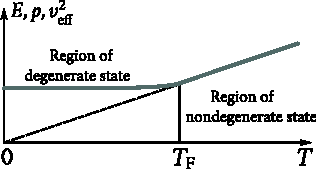
\includegraphics[scale=1]{figures/ch_03/fig_3_7.pdf}
		\caption[]{Temperature dependence of energy, pressure, and the square of effective velocity of electrons in a metal.}
		\label{fig:3_7}
	\end{center}
	\vspace{-0.7cm}
\end{figure}

In conclusion, to illustrate the drastic difference in the behaviour of the ideal nondegenerate gas obeying the Maxwell-Boltzmann statistics and of the degenerate electron gas described by the Fermi-Dirac statistics, we would like to cite some of their properties (\tab{3_3}).

\begin{table}[!b]
	\renewcommand{\arraystretch}{1.2}
	\caption{}
	\vspace{-0.6cm}
	\label{table:3_3}
	\begin{center}\resizebox{0.9\linewidth}{!}{
			\begin{tabular}{lll}
				\toprule[1pt]
				\multirow{2}{*}{\textbf{Parameters}} & \multicolumn{2}{c}{\textbf{Gas}}\\
                \cline{2-3}
                & \textbf{Nondegenerate} & \textbf{Degenerate}\\
				\midrule[0.5pt]\midrule[0.5pt]
                $\overline{E}$ at \SI{0}{\kelvin} & $0$ & $\overline{E}_0=\frac{3}{5}\ab{E}{F}$\\
                $\overline{E}$ at $T$ \si{\kelvin} & $\overline{E}=\frac{3}{2}\ab{k}{B}T$ & $\overline{E}=\frac{3}{5}\ab{E}{F}\bracket{1+\frac{5\pi^2}{12}\parenthesis{\frac{\ab{k}{B}T}{\ab{E}{F}}}^2}\approx\frac{3}{5}\ab{E}{F}$\\
                $\ab{v}{eff}$ at \SI{0}{\kelvin} & $0$ & $\ab{v}{eff,$0$}=\parenthesis{\frac{\ab{E}{F}}{m}}^{1/2}\approx\SI{e6}{\metre\per\second}$\\
                $\ab{v}{eff}$ at $T$ \si{\kelvin} & $\ab{v}{eff}=\parenthesis{\frac{3\ab{k}{B}T}{m}}^{1/2}$ & $\ab{v}{eff}=\ab{v}{eff,,$0$}$\\
                $p$ at \SI{0}{\kelvin} & $0$ & $p_0=\frac{2}{3}\overline{E}_0\approx\SI{e10}{\pascal}$\\
                $p$ at $T$ \si{\kelvin} & $p=\frac{RT}{V}$ & $p\approx p_0$\\
				\bottomrule[1pt]
			\end{tabular}
	}\end{center}
\end{table}

It follows that average energy $\overline{E}$, effective velocity $\ab{v}{eff}$ and pressure $p$ of a nondegenerate ideal gas are functions of temperature that vanish at absolute zero. At the same time $\overline{E}$, and $p$ of a degenerate electron gas are very large already at absolute zero and are practically independent of temperature (\fig{3_7}). This points to the fact that, as noted above, $\overline{E}$, $\ab{v}{eff}$, and $p$ of a degenerate electron gas are for the most part not of thermal origin, the contribution of the thermal electron motion to these quantities being negligible.

\section{Distribution function for a degenerate boson gas}\label{sec:28}

In contrast to the electrons, which satisfy the Pauli exclusion principle, the bosons can occupy both the free states and the states already occupied by other bosons the more readily the greater the occupancy of the latter.

The distribution function of bosons over the states was first obtained by Bose and Einstein. It is of the following form:
\begin{equation}\label{eq:3_50}
    \ab{f}{Bose}(E) = \frac{1}{\bracket{e^{(E-\mu)/(\ab{k}{B}T)} - 1}}.
\end{equation}

\noindent
(An elementary derivation of this expression is given in Appendix \ref{sec:A_III}). It is termed the \textit{Bose-Einstein distribution function}. Let us use it to describe the state of a photon gas.

Suppose that a cavity inside a black body at a temperature $T$ is filled with equilibrium thermal radiation. From the quantum mechanical point of view this radiation may be regarded as consisting of an enormous number of photons constituting a photon gas. The photon's spin is $s=1$. Therefore, photons are bosons, which implies that the photon gas should satisfy the Bose-Einstein distribution.

The photons have some peculiarities as compared with other bosons, for instance, the helium nucleus, \enlevel{\frac{4}{2}}{He}{}:
\begin{enumerate}[(1)]
    \item The rest mass of a photon is zero.

    \item All photons move with the same speed equal to that of light, $c$, but can have different energy $E$ and momentum $p$; $E$ and $p$ depend on the photon's frequency:
    \begin{equation}\label{eq:3_51}
        E = h\nu = \hslash\omega,\quad p = \frac{h\nu}{c} = \frac{\hslash\omega}{c}
    \end{equation}

    \noindent
    where $\hslash=h/2\pi$ and $\omega=2\pi\nu$. It follows from \eqref{eq:3_51} that
    \begin{equation}\label{eq:3_52}
        E = pc.
    \end{equation}

    \item The photons do not collide with one another. Therefore, an equilibrium distribution in a photon gas can be established only in the presence of a body capable of absorbing and emitting photons. The walls of the cavity in which the radiation is contained may serve as an example of such a body. The transformation of a photon of one frequency into a photon of another frequency takes place in the processes of absorption and subsequent emission.

    \item The photons may be generated (in the act of emission) and annihilated (in the act of absorption) in any numbers. Therefore, the number of photons in a photon gas does not remain fixed but depends on the state of the gas. For specified values of $V$ and $T$ the photon gas in a state of equilibrium contains so many photons $N_0$ as are needed for the energy of the gas to be at its minimum. This makes it possible to express the condition for the equilibrium of the photon gas in the form:
    \begin{equation}\label{eq:3_53}
        \parenthesis{\diff{E}{N}}_{V,T} = 0.
    \end{equation}

    \noindent
    Since according to \eqref{eq:3_8} $(\diffin{E}{N})_{V,T}=\omega$ the equilibrium condition \eqref{eq:3_53} means that $\mu=0$. Hence, the chemical potential of an equilibrium photon gas is zero.
\end{enumerate}

For a nondegenerate gas the chemical potential is negative and has a relatively great absolute value. The fact that for the photon gas $\mu=0$ means that such gas is always degenerate.

Setting $\mu=0$ in \eqref{eq:3_50}, we obtain the distribution function for the photon gas:
\begin{equation}\label{eq:3_54}
    \ab{f}{P}(E) = \frac{1}{\bracket{e^{E/(\ab{k}{B}T)} - 1}} = \frac{1}{\bracket{e^{(\hslash\omega)/(\ab{k}{B}T)} - 1}}.
\end{equation}

\noindent
This formula was first obtained by Max Planck and is termed the \textit{Planck formula}. It represents the average fraction of photons having the energy $E=\hslash\omega$. Using this formula, we may easily formulate the law for the energy distribution in the spectrum of a black body. The following expression can be obtained for the energy density of the radiation of such a body:
\begin{equation}\label{eq:3_55}
    \rho(\omega) = \frac{2\hslash}{\pi c^3} \bracket{\frac{\omega^3}{e^{(\hslash\omega)/(\ab{k}{B}T)} - 1}}.
\end{equation}

The readers are requested to derive this formula themselves making use of \eqref{eq:3_54} and \eqref{eq:3_18}.

\section{Rules for statistical averaging}\label{sec:29}

As was already stated, to specify the state of an ensemble one should specify its state parameters. To specify the state of a particle one should specify the values of its coordinates and momentum components.

The problem of going over from the parameters of the individual particles to the state parameters characterizing the ensemble involves the problem of transition from the dynamical laws describing the behaviour of the individual particles to the statistical laws describing the behaviour of the ensemble. To effect such a transition it is necessary to perform the averaging of the characteristics of motion of the individual particles assuming the chances of all the particles belonging to the ensemble to be identical. The state parameters of the ensemble are expressed in terms of the averaged parameters of the individual particles belonging to the ensemble.

To make the rules of averaging apparent, let us consider an ensemble of $N$ identical particles each of which is capable of assuming one of the discrete set of energy values: $E_1, E_2,\ldots, E_m$. Choose an arbitrary moment of time and note the energy every particle has at that moment. We obtain as a result a set of numbers $N(E_i)$ expressing the number of particles having the energy $E_i$. To determine the average energy $\overline{E}$ of the particles we add up the energies of all of them and divide the sum by the number of particles. The total number of particles is $N=\sum_{i=1}^m N(E_i)$, and the sum of their energies is $\sum_{i=1}^m E_i N(E_i)$. Therefore,
\begin{equation}\label{eq:3_56}
    \overline{E} = \frac{\displaystyle\sum_{i=1}^m E_i N(E_i)}{\displaystyle\sum_{i=1}^m N(E_i)}.
\end{equation}

\noindent
The average value $E$ obtained in this fashion is termed an \textit{ensemble average}.

If the particle's energy assumes a continuous set of values, the practice is to count the number of particles having an energy lying within an interval ($E, E+\deriv{E}$) instead of the number of particles having an exact value of energy. The average energy will then be
\begin{equation}\label{eq:3_57}
    \overline{E} = \frac{\displaystyle\int_0^{\infty} E N(E)\, \deriv{E}}{\displaystyle\int_0^{\infty} N(E)\, \deriv{E}}.
\end{equation}

Such averaging may be performed for any physical quantity $M$ that is a function of the coordinates and the momenta of the particles making up the ensemble. If $M$ is continuous,
\begin{equation}\label{eq:3_58}
    \overline{M} = \frac{\displaystyle\int_0^{\infty} M N(M)\, \deriv{M}}{\displaystyle\int_0^{\infty} N(M)\, \deriv{M}}.
\end{equation}

Let us determine the average energy of the particles of an ideal nondegenerate gas. According to \eqref{eq:3_57} and \eqref{eq:3_28}, we have
\begin{equation}\label{eq:3_59}
    \overline{E} = \frac{\displaystyle\int_0^{\infty} E N(E)\, \deriv{E}}{\displaystyle\int_0^{\infty} N(E)\, \deriv{E}} = \frac{2}{\sqrt{\pi(\ab{k}{B}T)^3}} \int_0^{\infty} e^{-E/(\ab{k}{B}T)} E^{3/2}\, \deriv{E} = \frac{3}{2}\ab{k}{B}T.
\end{equation}

The results of the calculations  of the average values of the velocity, of a velocity component, of the effective velocity, and of its component for the particles of an ideal gas are presented thus:
\begin{align*}
    \overline{v} &= \parenthesis{\frac{8\ab{k}{B}T}{\pi m}}^{1/2},\quad \overline{v}_x = \parenthesis{\frac{\ab{k}{B}T}{2\pi m}}^{1/2},\\
    \ab{v}{eff} &= \parenthesis{\frac{3\ab{k}{B}T}{m}}^{1/2},\quad \ab{v}{eff,$x$} = \parenthesis{\frac{\ab{k}{B}T}{m}}^{1/2}.
\end{align*}

The reader may for the sake of practice perform these calculations himself.
